\documentclass[a4,center,fleqn]{NAR}
\usepackage{lipsum}

% Enter dates of publication
\copyrightyear{XXXX}
\pubdate{XX XXXX XXXX}
\pubyear{XXXX}
\jvolume{XX}
\jissue{XX}

\articlesubtype{This is a draft}

\begin{document}

\title{???}

\author{%
Rodrigo Vargas Honorato\,$^{1,2}$,
Jorge Roel Touris\,$^{1}$
Alexandre Bonvin\,$^1$%
\footnote{To whom correspondence should be addressed.
Tel: +44 000 0000000; Fax: +44 000 0000000; Email: xxx@yyyy.ac.zz}}

\address{%
$^{1}$Bijvoet Center for Biomolecular Research, Faculty of Science, Utrecht University, Utrecht 3584CH, the Netherlands
$^{2}$Brazilian Biosciences National Laboratory (LNBio), Brazilian Center for Research in Energy and Materials (CNPEM), Zip Code 13083-970, Campinas, Sao Paulo, Brazil.}
% Affiliation must include:
% Department name, institution name, full road and district address,
% state, Zip or postal code, country

\history{%
Received XXXX X, XXXX;
Revised XXXX X, XXXX;
Accepted XXXX X, XXXX}

\maketitle

\begin{abstract}
\lipsum[1-1]

\end{abstract}


\section{Introduction}

Computational modeling of protein structures, interactions and dynamics has been advancing steadily in the past decades. Nonetheless researchers still face challenges when modeling large biomolecular systems with. Reducing the representation level from all-atom to coarse-grained is a way to bypass limitations such as algorithmic efficiency and available computing power [10.1016/j.cub.2010.11.06].

The main objective of a coarse-grained representation is to reduce the degrees of freedom, replacing amino acids (either fragments or entire side chains) with pseudo-atoms. The first coarse-grained protein models were built in the 70's and were successfully able to simulate an entire folding process [10.1038/253694a0]. Further development of the model accounted for the variable orientation of the pseudo sidechains and torsional potential for the main chain degrees of freedom were based on the statistical analysis of conformational properties of dipeptides [10.1016/0022-2836(76)90004-8]. 

Since proteins adopt a well-defined three-dimensional arrangement defined by both the conformational restraints of the main-chain as well as interactions with the environment by the side chains, it is expected that a coarse-grained representation of a protein contains all its crucial elements. The main objective of this representation is to reduce the number of degrees of freedom inherent to a protein structure. 

% How this can be used for docking?

The development of coarse-grained force fields have taken two directions; physics-based, following the same philosophy of it full-atom counterpart, basing it on molecular physics and knowledge-based that takes advantage the growing databases via statistical analysis. Here we apply the knowledge-based forcefield CG MARTINI [10.1021/jp071097f] which has been extended to account for nucleic-acids [10.1021/acs.jctc.5b00286], in our data-driven docking program HADDOCK <ref>. Whilst there are some CG docking algorithms for protein-protein <ref attract, pydockcg, haddock> the approach has nos been applied protein-DNA before.

We demonstrate this feature by modeling the polycomb repressive complex 1 (PRC1) in complex with its nucleosome core particle substrate. PRC1 is assembled as a multi-component arrangement which is responsible for chromatin structure remodeling both directly and through the establishment and removal of histone post-translational modifications [10.1038/nature13890].

% **************************************************************
% Keep this command to avoid text of first page running into the
% first page footnotes
\enlargethispage{-65.1pt}
% **************************************************************


\section{MATERIALS AND METHODS}

\subsection{HADDOCK-MARTINI integration}
The MARTINI CG DNA model was systematically parametrized according to the MARTINI philosophy, being backwards compatible with all other MARTINI model implementations. Experimental values such as liquid densities and partitioning free energies of small solutes between polar and non polar solvents are used to determine non-bonded interaction parameters[10.1021/acs.jctc.5b00286].

The parametrization used by Uusitalo and collaborators combines top-down (experimental data) and bottom-up (atomistic simulations) methodologies to parametrize the CG DNA model. The CG bead types for each nucleobase were selected based on partition free energies from water to chloroform or hydrated octanol. Bonded interactions have been fitted to reproduce dihedral, angle and bond distributions from atomistic simulation of short single stranded DNAs (ssDNAs).

The HADDOCK-MARTINI integration was done in accordance to the CG protein-protein implementation [\textbf{Jorge 2019}] with exception of the definition of new CG chemical types and a novel patch, both to account for the Watson-crick pairing.

\subsection{Protein-DNA Benchmark}
To evaluate and compare the speed increase and success rates of the CG protein-DNA docking implementation the protein-DNA benchmark v1.2 [10.1093/nar/gkn386] was used. This benchmark is composed of 47 unbound-unbound test cases that cover all major protein-DNA complexes [10.1186/gb-2000-1-1-reviews001] with an average of 3934 atoms. Complexes with modified nucleic bases were removed from the test set since there is no available CG topological information (1DFM, 1DIZ, 1EMH, 4KTQ). 

\subsection{Docking procedure}
The conversion of the atomic PDB coordinate file containing DNA/protein to CG is done via an improved version of the current aa2cg.py script used for pre-processing input structures for CG protein-protein docking [Jorge 2019]. Since the MARTINI forcefield has different parameters for bead involved in base-pairing, the atoms mapping to these beads must be correctly identified. This is done by checking atomic distances of atoms involved in the Watson-crick pairing and of the phosphates to ensure that the only opposite nucleotides are identified. 

Docking simulations were performed using optimal parameters for Protein-DNA [10.1093/nar/gkq222], the dieletric constant ($\epsilon$) is set to 78.0 during rigid-body and semi-flexible refinement in order to implicitly mimic the polarisability of water and changed back to 1.0 for water refinement. % what about desolv=0.0?
Sampling was kept to default 1000/200/200 for each docking stage (it0, it1, water) and ambiguous interaction restraints (AIR) were generated based on the true interfaces of the complexes. This was done in accordance to the previous full-atom protein-DNA benchmarking [10.1093/nar/gkq222] and converted to CG: (1) intermolecular atomic contacts below 5.0 \AA; (2) separated in three categories, amino-acid - nucleotide base, amino-acid - nucleotide backbone and amino-acid full nucleotide contact; (3) discarding amino-acid residues with relative main or side-chain solvent accessibility higher than 30 \% according to NACCESS [ref]. 

\subsection{Model evaluation}
Models were evaluated on each stage of docking using on the interface root mean square deviation (i-rmsd), calculated over the backbone CG beads (it0, it1) and AA atoms (water) using PROFIT [ref]. In accordance to the standard CAPRI metrics, models with i-RMSD $\leq 4.0$ \AA, $\leq 2.0$ \AA and $\leq 1.0$ \AA were considered as having acceptable, medium and high quality accordingly. The success rate, a measure of how many models are found within a specific range and below the acceptable threshold, was also evaluated. Ranges selected for this evaluation were top1, top5, top100, top400 and top1000 (it0, it1).

\subsection{Coarse grain docking of the PRC1 complex}
% talk to Alex about what would be relevant here

\section{RESULTS}

\subsection{Protein-DNA CG Docking perfomance}
Quality of both CG and AA docking were evaluated by calculating the interface RMSD of the generated solutions against the bound conformation of each target in the filtered testset (n=43). A comparison of this metric rate during the rigid body stage revealed that the CG protocol underperformed by 9.3 \% for the top1 model, 4.6 \% in top5 and top100 and 2.3 \% in both top400 and top1000. In the semi-flexible stage the AA protocol had a 39.53 \% higher success rate for top1, 20.93 \% for top5 and 4.65 \% for top100, top400 and top1000. % why? % 
CG models are mapped back to AA before going into the water refinement stage as described previously [Jorge 2019], our analysis showed this refinement greatly normalizes success rate differences, in which 4.65 \% was observed for top1, 2.3 \% for top5 and no difference for the remaining ranges (Figure ~\ref{it0}).

Reducing degrees of freedom makes the docking task computationally more efficient. The average computational time to generate one AA model in it0 and it1 was 44.3s and 270.43s respectively, whereas for CG this calculation was done in 8.8s and 38.1s. The implementation of the MARTINI CG beads for Protein-DNA docking in this dataset revealed a 4-fold increase during rigid-body docking and a 7-fold increase during semi-flexible stage. % why not same on both?

\begin{figure}[t]
\begin{center}
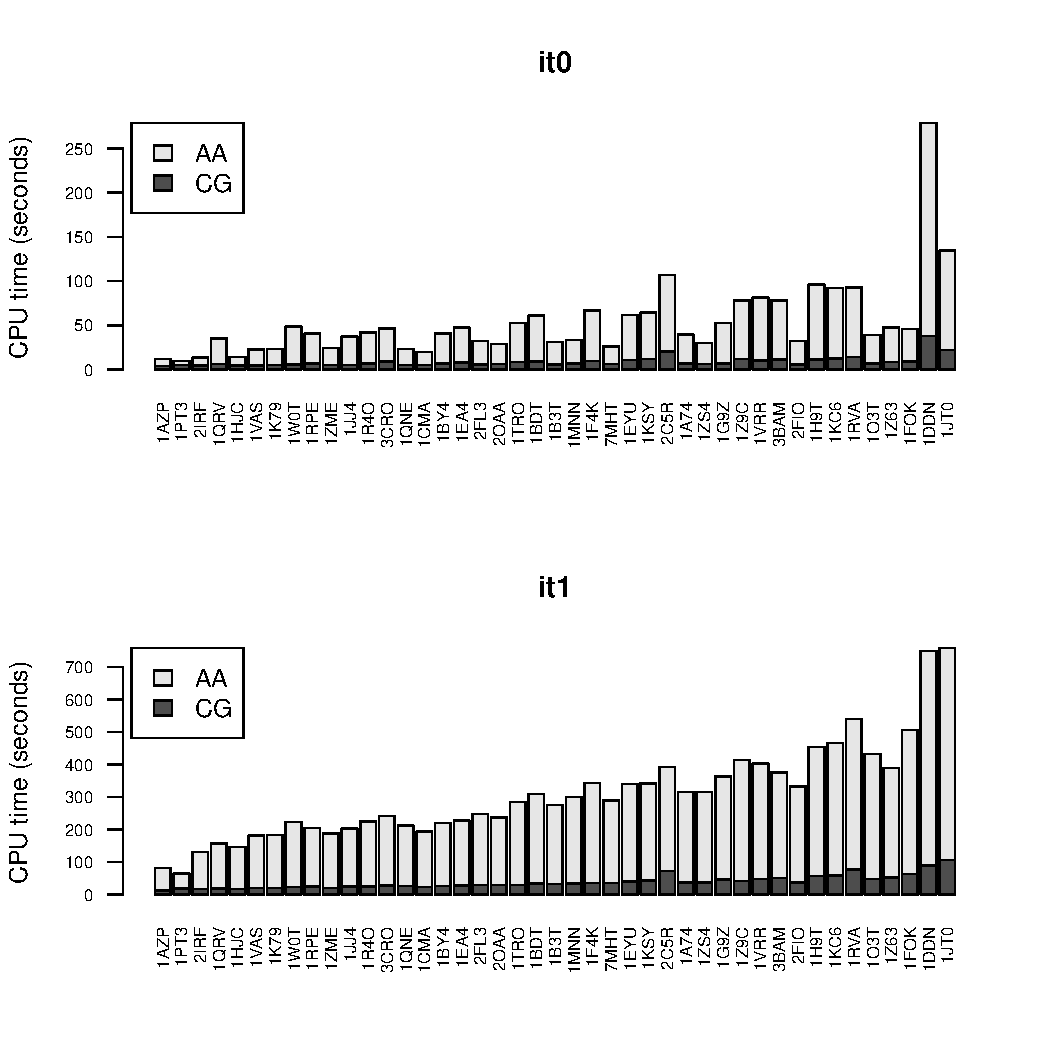
\includegraphics[width=0.5\textwidth]{figures/cpu-time.pdf}
\end{center}
\caption{Computing time (models/second) comparison for rigid-body (A) and semi-flexible (B) stages of all-atom and coarse grained Protein-DNA docking.}
\label{cpu-time}
\end{figure}

\subsection{Coarse grain docking of the PRC1 complex}

\section{DISCUSSION}

\subsection{Discussion subsection one}

\section{CONCLUSION}


\section{ACKNOWLEDGEMENTS}

Grant was provided by FAPESP (2017/03191-2) and funding ...


\subsubsection{Conflict of interest statement.} None declared.
\newpage


%\bibliography{DNA-CG-Draft} % does not work
\begin{thebibliography}{4}

% Format for article
\bibitem{1}
Author,A.B. and Author,C. (1992)
Article title.
\textit{Abbreviated Journal Name}, \textbf{5}, 300--330.

% Format for book
\bibitem{2}
Author,D., Author,E.F. and Author,G. (1995)
\textit{Book Title}.
Publisher Name, Publisher Address.

% Format for chapter in book
\bibitem{3}
Author,H. and Author,I. (2005)
Chapter title.
In
Editor,A. and Editor,B. (eds),
\textit{Book Title},
Publisher Name, Publisher Address,
pp.\ 60--80.

% Another article
\bibitem{4}
Author,Y. and Author,Z. (2002)
Article title.
\textit{Abbreviated Journal Name}, \textbf{53}, 500--520.

\end{thebibliography}

\end{document}
